\subtitle{Konstituentenreihenfolge}

\huberlintitlepage[22pt]

%\if0
\section{Konstituentenreihenfolge}

\iftoggle{teil1}{
\outline{

\begin{itemize}
\item Ziele
\item Formalismus
\item Valenz und Grammatikregeln
\item Dominanzstrukturen und Prinzipien
\item Semantik
\item Adjunktion und Spezifikation
\item Das Lexikon: Typen und Lexikonregeln
\item Topologie des deutschen Satzes
\item \blau{Konstituentenreihenfolge}
\item Nichtlokale Abhängigkeiten
\item Relativsätze
%\item Komplexe Prädikate: Der Verbalkomplex
\end{itemize}
}

} % \end{teil1}

\iftoggle{teil2}{
\outline{
\begin{itemize}
\item Wiederholung
      \begin{itemize}
\item Wozu Syntax? / Phrasenstrukturgrammatiken
\item Formalismus
\item Valenz und Grammatikregeln
\item Dominanzstrukturen und Prinzipien
\item Semantik
\item Topologie des deutschen Satzes
\item \blau{Konstituentenreihenfolge}
\item Nichtlokale Abhängigkeiten
\end{itemize}
\item Kongruenz
\item Kasus
\item Der Verbalkomplex
\item Kohärenz, Inkohärenz, Anhebung und Kontrolle
\item Passiv
\item Partikelverben
\item Morphologie
\end{itemize}
}
} % \end{teil2}

%\if0
\frame{
\frametitle{Literaturhinweise}
%
\begin{itemize}
\item Literatur: \citew[Kapitel~9.1--9.4]{MuellerLehrbuch3} %sowie \citew[Kapitel~9.5.1]{MuellerLehrbuch3}

\item Handbuchartikel: \citew{MuellerOrder}

\item Buch zur deutschen Satzstruktur:\\
      \citew{MuellerGS} auf der Grundlage von \citew{Mueller2005c,Mueller2005d}
\end{itemize}

% \vspace{1cm}

% Damit alles kompatibel zum Lehrbuch bleibt,\\
% nehmen wir hier auch das \subcatm für die Valenz an.

% \subcat = \spr + \comps

% Zu neueren Versionen der HPSG, die \subcat in \spr und \comps unterteilen,\\ siehe
% \citew{Sag97a,HPSGHandbook,MuellerGermanic}.

% Deutsch: Argumente von finiten Verben sind alle auf \comps,\\
% so dass die Verwendung von \subcat hier keinen Unterschied macht.


%% \rotbf{Achtung, wichtiger Hinweis: Diese Literaturangabe hier bedeutet,\\dass Sie die Literatur zum
%%   nächsten Mal lesen sollen!!!!}
}


\iftoggle{teil1}{
\frame{
\frametitle{Konstituentenstellung}

\savespace
\begin{itemize}[<+->]
\item Deutsch ist eine Sprache mit relativ freier Konstituentenstellung.
\item Das Deutsche wird typologisch zu den Verbletztsprachen (SOV) gezählt.\\
In deklarativen Hauptsätzen und in Fragesätzen steht das Verb jedoch\\an zweiter
bzw.\ an erster Stelle. 
\item Wie kann man die Umstellung von Argumenten erklären?
\item Wie lassen sich die verschiedenen Verbstellungen erfassen?
\end{itemize}

}
} % \end{teil1}



\subsection{Anordnung von Konstituenten im Mittelfeld}

\subsubsection{Argumente}

\frame{
\frametitle{Relativ freie Konstituentenstellung}

\begin{itemize}
\item Im \mf können Argumente in nahezu beliebiger Abfolge angeordnet werden.
\eal
\ex weil \rot{der Delphin} \gruen{dem Kind} \blau{den Ball} gibt
\ex weil \rot{der Delphin} \blau{den Ball} \gruen{dem Kind} gibt
\ex weil \blau{den Ball} \rot{der Delphin} \gruen{dem Kind} gibt
\ex weil \blau{den Ball} \gruen{dem Kind} \rot{der Delphin} gibt
\ex weil \gruen{dem Kind} \rot{der Delphin} \blau{den Ball} gibt
\ex weil \gruen{dem Kind} \blau{den Ball} \rot{der Delphin} gibt
\zl
\pause
\item In (\mex{0}b--f) muss man die Konstituenten anders betonen
und die Menge der Kontexte, in denen der Satz mit der jeweiligen Abfolge
geäußert werden kann, ist gegenüber (\mex{0}a) eingeschränkt \citep{Hoehle82a}. 

Abfolge in (\mex{0}a) = \blau{Normalabfolge} bzw.\ die \blau{unmarkierte Abfolge}.
\end{itemize}
}

\subsubsection{Adjunkte}
\frame{
\frametitle{Adjunkte im Mittelfeld}

%\savespace
\begin{itemize}
\item Außer Argumenten können sich noch Adjunkte im \mf befinden. 
\pause
\item Diese können an beliebigen Positionen zwischen Argumenten stehen:
\eal
\ex weil \blau{morgen} der Delphin den Ball dem Kind gibt
\ex weil der Delphin \blau{morgen} den Ball dem Kind gibt
\ex weil der Delphin den Ball \blau{morgen} dem Kind gibt
\ex weil der Delphin den Ball dem Kind \blau{morgen} gibt
\zl
\pause
\item Skopustragende Adjunkte kann man im Mittelfeld nicht umordnen,\\
ohne die Bedeutung des Satzes zu ändern:
\eal
\ex weil er absichtlich nicht lacht
\ex weil er nicht absichtlich lacht
\zl
\end{itemize}
}

\frame{
\frametitle{Analysen}

\begin{itemize}[<+->]
\item große Anzahl alternativer Vorschläge zur Erklärung der Daten 
\item Bei Behandlung der Mittelfeldabfolgen spielt immer auch die Behandlung der Verbstellung eine Rolle. 
\item Wichtig für die Auswahl des richtigen Ansatzes sind bestimmte Arten von Vorfeldbesetzung. 
\item Die entsprechenden Teilanalysen werden später behandelt,\\
      so dass es erst dann möglich ist, alternative Analysen zu besprechen.
\end{itemize}
}

\frame{
\frametitle{Binär verzweigende Strukturen}

\begin{itemize}
\item Sätze wie (\mex{1}) sind kein Problem:
\ea
weil [der Delphin [den Ball [dem Kind gibt]]]
\z
\pause
\item Die Integration von Adjunkten ist ebenfalls unproblematisch:
\eal
\ex weil [\blau{morgen} [der Delphin [den Ball [dem Kind gibt]]]]
\ex weil [der Delphin [\blau{morgen} [den Ball [dem Kind gibt]]]]
\ex weil [der Delphin [den Ball [\blau{morgen} [dem Kind gibt]]]]
\ex weil [der Delphin [den Ball [dem Kind [\blau{morgen} gibt]]]]
\zl
\pause
\item Die unterschiedliche Bedeutung der Sätze in (\mex{1})
ergibt sich aus Unterschied in Einbettung.
\eal
\ex weil er [absichtlich [nicht lacht]]
\ex weil er [nicht [absichtlich lacht]]
\zl

\end{itemize}

}

\subsubsection{Argumente}

\frame{
\frametitle{Permutation der Argumente im \mf}


\begin{itemize}
\item Permutation der Argumente ist noch nicht erklärt
\pause
\item bisher immer Kombination des Kopfes mit dem letzten Argument:
\label{schema-bin}
\type{head-argument-phrase} \impl\\*
\onems{
      subcat \ibox{1} \\
      head-dtr$|$subcat \ibox{1} $\oplus$ \sliste{ \ibox{2} } \\
      non-head-dtrs \sliste{ \ibox{2} }\\
      }
\pause
\item Verallgemeinerung des Kopf"=Argument"=Schemas:\\
      Statt die \subcatl in zwei Listen zu teilen, zerteilen wir sie in drei.\\
      So wird es möglich, ein Element aus der Mitte oder auch vom Rand zu nehmen:
\ibox{1} $\oplus$ \sliste{ \ibox{2} } $\oplus$ \ibox{3}
\end{itemize}
}

\frame{
\frametitle{Das Kopf-Argument-Schema}

\begin{itemize}
\item bisherige Version:\\
\type{head-argument-phrase} \impl\\*
\onems{
      cat$|$subcat \ibox{1} \\
      head-dtr$|$cat$|$subcat \ibox{1} $\highlight{\oplus}$ \sliste{ \ibox{2} } \\
      non-head-dtrs \sliste{ \ibox{2} }\\
      } \\
\item revidierte Version für Deutsch:\\
{\it head-argument-phrase\/} \impl\\
\onems{
      subcat \ibox{1} $\oplus$ \ibox{3}\\
      head-dtr$|$subcat \ibox{1} $\oplus$ \sliste{ \ibox{2} } $\oplus$ \ibox{3}\\
      non-head-dtrs \sliste{ \ibox{2} }\\
      }

\end{itemize}
}

\frame{
\frametitle{Beispiel: Normalabfolge}
\eal
\ex weil niemand den Roman kennt
\ex weil den Roman niemand kennt
\zl


\centerline{%
\begin{forest}
sm edges
[{V[\subcat \eliste]}
  [{\ibox{1} NP[\textit{nom}]}
    [niemand]]
  [{V[\subcat \nliste{ \ibox{1} }]}
    [{\ibox{2} NP[\type{acc}]}
       [den Roman,roof]]
    [{V[\subcat \nliste{ \ibox{1}, \ibox{2} } ]}
      [kennt]]]]
\end{forest}}

}

\frame{
\frametitle{Beispiel: Umstellung}


\centerline{%
\begin{forest}
sm edges
[{V[\subcat \eliste]}
  [{\ibox{2} NP[\type{acc}]}
     [den Roman,roof]]
  [{V[\subcat \nliste{ \ibox{2} }]}
    [{\ibox{1} NP[\textit{nom}]}
      [niemand]]
    [{V[\subcat \nliste{ \ibox{1}, \ibox{2} } ]}
      [kennt]]]]
\end{forest}}

\medskip
Unterschied nur in Abbindungsreihenfolge der Elemente in \subcat
}


\iftoggle{teil1}{
\subsection{Linearisierungsregeln}

\frame[shrink=10]{
\frametitle{Linearisierungsregeln}

%\smallframe
\savespace
\begin{itemize}
\item Regelschemata sind abstrakte Repräsentationen,\\
      die nur etwas über die Bestandteile einer Phrase (unmittelbare Dominanz) aussagen,\\
      nicht jedoch über die Abfolge von Töchtern (lineare Präzendenz\is{Präzedenz}) 
\pause
\item Trennung zwischen \emph{immediate dominance} (ID)
und \emph{linear precedence} (LP) schon in der \gpsg \citep*{GKPS85a}
\pause
\item Motivation: Permutation mit Phrasenstrukturregeln $\to$\\
braucht für ditransitive Verben sechs Phrasenstrukturregeln für Verbletztstellung:
\ea
\begin{tabular}[t]{l@{ }l@{ }l@{ }l@{ }l@{ }}
S  & $\to$ NP[nom],& NP[acc], & NP[dat], & V\\
S  & $\to$ NP[nom],& NP[dat], & NP[acc], & V\\
S  & $\to$ NP[acc],& NP[nom], & NP[dat], & V\\
S  & $\to$ NP[acc],& NP[dat], & NP[nom], & V\\
S  & $\to$ NP[dat],& NP[nom], & NP[acc], & V\\
S  & $\to$ NP[dat],& NP[acc], & NP[nom], & V\\
\end{tabular}
\z
\end{itemize}

}

\frame[shrink]{
\frametitle{Abstraktion von linearer Abfolge}

\begin{itemize}
\item Plus sechs Regeln für Verberststellung:
\medskip

\begin{tabular}[t]{@{}l@{ }l@{ }l@{ }l@{ }l}
S  & $\to$ V, NP[nom],& NP[acc], & NP[dat]\\
S  & $\to$ V, NP[nom],& NP[dat], & NP[acc]\\
S  & $\to$ V, NP[acc],& NP[nom], & NP[dat]\\
S  & $\to$ V, NP[acc],& NP[dat], & NP[nom]\\
S  & $\to$ V, NP[dat],& NP[nom], & NP[acc]\\
S  & $\to$ V, NP[dat],& NP[acc], & NP[nom]\\
\end{tabular}

\medskip

Die Regeln erfassen eine Generalisierung nicht.
\pause
\item \citet*{GKPS85a}:\\
      Trennung von unmittelbarer Dominanz  und linearer Abfolge 
\pause
\item Dominanzregeln sagen nichts über die Reihenfolge der Töchter.
\pause
\item LP"=Beschränkungen über lokale Bäume, \dash Bäume der Tiefe eins
\pause
\item statt zwölf Regeln nur noch eine + Aufhebung der Anordnungsrestriktion für die rechte Regelseite

\begin{tabular}[t]{@{}l@{ }l}
S  & $\to$ V NP[nom] NP[acc] NP[dat]\\
\end{tabular}

\end{itemize}
}

\frame{
\frametitle{Erneute Formulierung von Restriktionen}


\begin{itemize}
\item ohne Restriktionen für die rechte Regelseite gibt es zu viel Freiheit
\medskip
\begin{tabular}[t]{@{}l@{ }l}
S  & $\to$ V NP[nom] NP[acc] NP[dat]\\
\end{tabular}

\medskip
Die Regel lässt Abfolgen mit dem Verb zwischen NPen zu:
\ea[*]{
Der Delphin dem Kind gibt einen Ball.
}
\z
\pause
\item Linearisierungsregeln schließen solche Anordnungen dann aus.
\end{itemize}
}

\frame{
\frametitle{Konstituentenordnung in binär verzweigenden Strukturen}
\smallframe
\begin{itemize}
\item \begin{tabular}[t]{@{}ll@{}}
der Kopf kommt zuerst:                                   & Beispiel:\\
%
\ms{
phon & \blau{\ibox{1} $\oplus$ \ibox{2}}\\
head-dtr & \onems{ phon \ibox{1}}\\
non-head-dtrs & \liste{ \onems{ phon \ibox{2} }} \\
}&%
\ms{
phon & \phonliste{ schläft, Karl }\\
head-dtr & \onems{ phon \phonliste{ schläft } }\\
non-head-dtrs & \phonliste{ \onems{ phon \phonliste{ Karl } }} \\
}\\
\end{tabular}
\pause
\item \begin{tabular}[t]{@{}ll@{}}
der Kopf kommt zum Schluss:                            & Beispiel:\\
%
\ms{
phon & \blau{\ibox{2} $\oplus$ \ibox{1}}\\
head-dtr & \onems{ phon \ibox{1}}\\
non-head-dtrs & \liste{ \onems{ phon \ibox{2} }} \\
}&%
\ms{
phon & \phonliste{Karl, schläft }\\
head-dtr & \onems{ phon \phonliste{ schläft } }\\
non-head-dtrs & \liste{ \onems{ phon \phonliste{ Karl } }} \\
}\\
\end{tabular}
\end{itemize}
}

\frame{
\frametitle{Nötige Beschränkungen}

Bisher schließt nichts (\mex{1}) und (\mex{2}) aus:
\eal
\ex[*]{
{}[[den Schrank] in]
}
\ex[*]{
{}dass [er [es [gibt ihm]]]
}
\zl
\pause
\eal
\ex[*]{
dass [er [es [ihm [gibt nicht]]]]
}
\ex[*]{
{}[der [Mann kluge]]
}
\ex[*]{
{}[das [[am Wald] Haus]]
}
\zl
}

\frame{
\frametitle{Linearisierungsregeln in HPSG}

\begin{itemize}
\item LP-Regeln restringieren Reihenfolge von zwei beschriebenen Objekten.
\pause
\item verschiedene Arten von Linearisierungsregeln: 
      \begin{itemize}
      \item Bezug auf Merkmale der jeweiligen Objekte
\pause
      \item Bezug auf die syntaktische Funktion (Kopf, Komplement, Adjunkt, \ldots)
\pause
      \item Bezug auf beides
      \end{itemize}
\pause
\item Köpfe vs.\ Argumente:
\eal
\ex Head[\initial+] $<$ Argument
\ex Argument $<$ Head[\initial--]
\zl
\pause
\item Köpfe vs. Adjunkte:
\eal
\ex Adjunct[{\sc pre-modifier} +] $<$ Head
\ex Head $<$ Adjunct[{\sc pre-modifier} --]
\zl
\end{itemize}
}

\frame{
\frametitle{Konsequenzen der Linearisierungsregeln}

\small
nur noch die beiden folgenden Kopf"=Argument"=Strukturen werden lizenziert:

\onems{
phon \highlightbox{\ibox{1} $\oplus$ \ibox{2}}\\ 
cat$|$subcat \ibox{3} $\oplus$ \ibox{4}\\
head-dtr \ms{ phon & \ibox{1}\\
              cat  & \ms{ head$|$initial \highlightbox{+}\\
                          subcat \ibox{3} $\oplus$ \sliste{ \ibox{5} } $\oplus$ \ibox{4} \\
                        }\\
            }\\
non-head-dtrs \sliste{ \ibox{5} [ \phon \ibox{2} ] }\\
}

\pause
\onems{
phon \highlightbox{\ibox{2} $\oplus$ \ibox{1}}\\ 
cat$|$subcat \ibox{3} $\oplus$ \ibox{4}\\
head-dtr \ms{ phon & \ibox{1}\\
              cat  & \ms{ head$|$initial \highlightbox{$-$}\\
                          subcat \ibox{3} $\oplus$ \sliste{ \ibox{5} } $\oplus$ \ibox{4} \\
                        }\\
            }\\
non-head-dtrs \sliste{ \ibox{5} [ \phon \ibox{2} ] }\\
}

}

\frame{
\frametitle{Konsequenzen der Linearisierungsregeln: Beispiel}

\small
nur noch die beiden folgenden Kopf"=Argument"=Strukturen werden lizenziert:

\onems{
phon \highlightbox{\ibox{1} \phonliste{ schläft } $\oplus$ \ibox{2} \phonliste{ Karl }}\\ 
cat$|$subcat \ibox{3} $\oplus$ \ibox{4}\\
head-dtr \ms{ phon & \ibox{1} \phonliste{ schläft }\\
              cat  & \ms{ head$|$initial \highlightbox{+}\\
                          subcat \ibox{3} $\oplus$ \sliste{ \ibox{5} } $\oplus$ \ibox{4} \\
                        }\\
            }\\
non-head-dtrs \sliste{ \ibox{5} [ \phon \ibox{2} \phonliste{ Karl }] }\\
}

\pause
\onems{
phon \highlightbox{\ibox{2} \phonliste{ Karl } $\oplus$ \ibox{1} \phonliste{ schläft }}\\ 
cat$|$subcat \ibox{3} $\oplus$ \ibox{4}\\
head-dtr \ms{ phon & \ibox{1} \phonliste{ schläft }\\
              cat  & \ms{ head$|$initial \highlightbox{$-$}\\
                          subcat \ibox{3} $\oplus$ \sliste{ \ibox{5} } $\oplus$ \ibox{4} \\
                        }\\
            }\\
non-head-dtrs \sliste{ \ibox{5} [ \phon \ibox{2} \phonliste{ Karl } ] }\\
}

}


\subsection{Spezifikator-Kopf-Strukturen}

\frame{
\frametitle{Spezifikator-Kopf-Strukturen: NP-Strukturen?}

\ea
\label{ex-die-zerstoerung-der-stadt-dds}
die Zerstörung der Stadt durch die Soldaten
\z

Kopf-Argument-Schema würde eine der Anordnungen in (\mex{1}) erzwingen: 
\eal
\ex[*]{
Zerstörung die der Stadt durch die Soldaten
}
\ex[*]{
die der Stadt durch die Soldaten Zerstörung
}
\zl

Argumente, die von \emph{Zerstörung} abhängen müssen rechts stehen.
 
Nomina sind \textsc{initial}"=Wert `+'. Aber die Determinatoren?

DP-Analyse? 
\ea
{}[\sub{DP} [\sub{Det} die] [\sub{NP} [\sub{N} Zerstörung] [\sub{DP} der Stadt] [\sub{PP} durch die Soldaten]]]
\z
Nein, funktioniert nicht für Possessiva. \citep{MyPM2021a}

Englisch: Subjekt vor Verb + Objekten.

NP und Satz parallel mit Spezifikator-Kopf-Strukturen. 

}

\frame{
\frametitle{Komplexe NP-Struktur}

\vfill
\centerline{
\begin{forest}
sm edges
[N\feattab{\spr \eliste,\\
           \subcat \eliste}
  [\ibox{1} Det [die]]
  [N\feattab{\spr \sliste{ \ibox{1} },\\
           \subcat \eliste}
    [N\feattab{\spr \sliste{ \ibox{1} },\\
           \subcat \sliste{ \ibox{2} }}
      [N\feattab{\spr \sliste{ \ibox{1} },\\
           \subcat \sliste{ \ibox{2}, \ibox{3} }}
         [Zerstörung]]
      [\ibox{3} {NP[\type{gen}]}
        [der Stadt,roof]]]
    [\ibox{2} {PP[\type{durch}]}
      [durch die Soldaten,roof]]]]
\end{forest}}
\vfill

}

\frame[shrink]{
\frametitle{Spezifikator-Kopf-Schema}

\begin{schema}[Spezifikator-Kopf-Schema]\is{Schema!Spezifikator"=Kopf"=}
\label{schema-spr-h}
\type{head-specifier"=phrase}\istype{head"=specifier"=phrase} \impl\\
\onems{
      cat$|$spr \ibox{1} \\
      head-dtr$|$cat  \ms{ spr    & \ibox{1} $\oplus$ \sliste{ \ibox{2} } \\
                           subcat & \eliste \\
                         }\\
      non-head-dtrs \sliste{ \ibox{2} }\\
      }
\end{schema}

\noindent
\ea
\catw von \emph{Zerstörung}:\\
\ms{ head & \ms[noun]{ initial & $+$\\
                     }\\
     spr & \sliste{ Det }\\
           subcat & \sliste{ NP[\type{gen}], PP[\type{durch}] }\\[2mm]
         }
\z

Linearisierungsregel:
\ea
Specifier $<$ Head
\z

}


\frame{
\frametitle{Valenzprinzip}

Gegenstück zum Typ \type{head"=non"=argument"=phrase}: Typ \type{head"=non"=specifier"=phrase}:
\ea
\label{def-head-non-spr-phrase}
\type{head"=non"=specifier"=phrase}\istype{head"=non"=specifier"=phrase} \impl
\onems{
      cat$|$spr \ibox{1} \\
      head"=dtr$|$cat$|$spr \ibox{1}\\
      }
\z

}



\frame{
\frametitle{Typhierarchie}

\type{head"=argument"=phrase} und \type{head"=adjunct"=phrase} sind
Untertypen von \type{head"=non"=specifier"=phrase}:\\
\sprw der Kopf"|tochter ist mit dem \sprw der Mutter identisch.

\vfill
\centerline{\scalebox{.8}{%
\begin{forest}
type hierarchy,
% for tree={
%   calign=fixed angles,
%   calign angle=60,
% }, 
 for tree={l+=\baselineskip},
 for level={3}{l+=\baselineskip},
[phrase
    [non-headed-phrase]
    [headed-phrase
      [head-non-adjunct-phrase
        [head-adjunct-phrase,edge to=!uu2,edge to=!uu3,no edge]]
      [head-non-argument-phrase
       [head-argument-phrase,edge to=!uu1,edge to=!uu3, no edge]]
      [head-non-specifier-phrase
       [head-specifier-phrase,edge to=!uu1,edge to=!uu2, no edge]]]]
\end{forest}}}
\vfill

}

\subsection{Verberststellung}


% \frame{
% \frametitle{Verberststellung}
% %
% \begin{itemize}
% \item Literatur: \citew[Kapitel~9.4]{MuellerLehrbuch3}
% \end{itemize}


% \vspace{1cm}

% %% \rotbf{Achtung, wichtiger Hinweis: Diese Literaturangabe hier bedeutet,\\dass Sie die Literatur zum
% %%   nächsten Mal lesen sollen!!!!}
% }


\frame{
\frametitle{Verberststellung: Das Deutsche als SOV-Sprache}

\savespace
\begin{itemize}
\item Transformationsgrammatik und GB: Deutsch ist SOV"=Sprache\\
      \dash, Stellung Subjekt Objekt Verb wird als Normalstellung betrachtet\\
(\citealp{Bach62a}; \citealp{Bierwisch63a}; \citealp{Reis74a}; \citealp{Thiersch78a})\nocite{Fourquet57a,Fourquet70a}
\pause
\item V1- und V2-Sätze gelten als aus Verbletztsätzen durch Umstellung\\
      des finiten Verbs abgeleitet:
\eal
\ex dass er ihr gestern den Ball gegeben \highlight{hat}
\ex \highlight{Hat} er ihr gestern den Ball gegeben?
\ex Er \highlight{hat} ihr gestern den Ball gegeben.
\zl
(Wobei V2 = V1 + Voranstellung einer Konstituente)
\pause
\item Ähnliche Ansätze gibt es auch innerhalb der \gpsg \citep{Jacobs86a}\ia{Jacobs}
und innerhalb der HPSG (\citealp*{KW91a}\iaf{Kiss}\iaf{Wesche}; \citealp*{Netter92}\iaf{Netter}; \citealp{Oliva92a}; 
\citealp*{Kiss93}; \citealp*{Frank94}\iaf{Frank}; \citealp*{Kiss95a}; \citealp{Meurers2000b}; \citealp{Mueller2005c,Mueller2005d,MuellerGS}).
\end{itemize}
}

\subsubsection{Motivation der Verbletztstellung als Grundstellung}

\frame{
\frametitlefit{Motivation der Verbletztstellung als Grundstellung: Partikeln}

\citew%[S.\,34--36]
{Bierwisch63a}: Verbpartikel bilden mit dem Verb eine enge Einheit.
\eal
\ex weil er morgen \blau{anfängt}
\ex Er \blau{fängt} morgen \blau{an}.
\zl
Diese Einheit ist nur in Verbletztstellung zu sehen: Argument für Grundstellung
}



\frame{
\frametitle{Stellung von Idiomen}

\eal
\judgewidth{?*}
\ex[]{
dass niemand dem Mann den Garaus macht
}
\ex[?*]{
dass dem Mann den Garaus niemand macht
}
\ex[]{
Niemand macht ihm den Garaus.
}
\zl

Idiomteile wollen nebeneinader stehen (\mex{0}a,b).

Umstellung des Verbs ist abgeleitete Stellung. Nur zur Markierung des Satztyps.


}

\frame{
\frametitle{Stellung in Nebensätzen}

Verben in infiniten Nebensätzen und in durch eine Konjunktion eingeleiteten
finiten Nebensätzen stehen immer am Ende\\
(von Ausklammerungen ins Nachfeld abgesehen):
\eal
\ex Der Clown versucht, Kurt-Martin die Ware \blau{zu geben}.
\ex dass der Clown Kurt-Martin die Ware \blau{gibt}
\zl
}


\frame{
\frametitle{Stellung der Verben in SVO und SOV-Sprachen}

\citet{Oersnes2009b}: 
\eal
\ex dass er ihn gesehen$_3$ haben$_2$ muss$_1$
\ex 
\gll at han må$_1$ have$_2$ set$_3$ ham\\
     dass er muss haben sehen ihn\\
\zl
\pause

Nur das finite Verb wird umgestellt, die anderen Verben bleiben hinten:
\eal
\ex Muss er ihn gesehen haben?
\ex 
\gll Må han have set ham?\\
     muss er haben sehen ihn\\
\zl


}

\frame{
\frametitle{Skopus}

\citew[Abschnitt~2.3]{Netter92}:
Skopusbeziehungen der Adverbien hängt von ihrerer Reihenfolge ab (Präferenzregel?):\\
Links stehendes Adverb hat Skopus über folgendes Adverb und Verb.

\eal
\ex weil er [absichtlich [nicht lacht]]
\ex weil er [nicht [absichtlich lacht]]
\zl
\pause
Bei Verberststellung ändern sich die Skopusverhältnisse nicht.
\eal
\ex Lacht er absichtlich nicht?
\ex Lacht er nicht absichtlich?
\zl
}

\subsubsection{Analyse der Verberststellung}

\frame{
\frametitle{Parallele Strukturen für V1 und VL}

\eal
\ex weil er [absichtlich [nicht lacht]]
\ex weil er [nicht [absichtlich lacht]]
\zl

Nimmt man an, dass VL-Sätze eine parallele Struktur haben,\\
dann ist diese Tatsache automatisch erklärt. 

\pause
Annahme: leeres Element, das den Platz des Verbs in (\mex{0}) füllt und das bis auf den phonologischen Beitrag,
identisch mit dem normalen Verb ist, \dash, es hat dieselbe Valenz und leistet auch denselben semantischen
Beitrag. 
\eal
\ex Lacht$_i$ er [absichtlich [nicht \_$_i$]]?
\ex Lacht$_i$ er [nicht [absichtlich \_$_i$]]?
\zl
Das leere Element (\highlight{Spur} oder \highlight{Lücke} gennannt) ist als \_$_i$
gekennzeichnet. Zugehörigkeit zum Verb \emph{lacht} wird durch gemeinsamen
Index markiert.

}



\frame{
\frametitle{Die Verbspur}


\ea
Kennt$_i$ niemand den Roman \_$_i$?\label{bsp-kennt-er-das-buch}
\z

Verbspur für \emph{kennt}:\\
\ms{
phon & \phonliste{}\\
cat  & \ms{ head & \ms[verb]{ vform & fin\\
                            }\\
            subcat & \sliste{ \npnom{}\ind{1}, \npacc{}\ind{2} }\\
          }\\
cont & \ms[kennen]{
       experiencer & \ibox{1}\\
       theme       & \ibox{2}\\
       }\\
}

Dieser Eintrag unterscheidet sich vom normalen Verb nur im \phonw.
}

\frame{
\frametitle{Eine erste Skizze der Analyse}

~\vfill
\centerline{
\begin{forest}
sm edges
[\blau<2>{V[\subcat \eliste]}
  [\blau<2>{V} [kennt]]
  [{V[\subcat \eliste]}
    [{\ibox{1} NP[\type{nom}]}
      [jemand]]
    [{V[\subcat \sliste{ \ibox{1} } ]}
      [{\ibox{2} NP[\type{acc}]}
        [den Roman, roof]]
      [{V[\subcat \sliste{ \ibox{1}, \ibox{2} } ]}
        [\trace]]]]]
\end{forest}}
\begin{itemize}
\item Kombination der Spur mit Argumenten folgt normalen Gesetzmäßigkeiten
\pause
\item Aber wodurch ist das Verb in Initialstellung lizenziert?
\end{itemize}

\vfill

}

\frame{
\frametitle{Der Status des Verbs in Erststellung}

\savespace
\begin{itemize}
\item Parallelität zwischen Komplementierer und Verb \citep{Hoehle97a}:
\eal
\ex \highlight{dass} [niemand den Roman kennt]
\ex \highlight{Kennt} [niemand den Roman \_$_i$]?
\zl
\emph{kennt} hat Kopfstatus und selegiert eine gesättigte Verbalprojektion mit Verbletztstellung.
\pause
\item Unterschied:\\
      Finite Verben in Initialstellung verlangen Projektion einer Verbspur,\\
      wohingegen Komplementierer Projektionen von overten Verben verlangen. 
\pause
\item Verbalprojektion, mit der \emph{kennt} kombiniert wird,\\
muss genau die zu \emph{kennt} gehörige Verbspur enthalten. 

Mit Verbspur für \emph{gibt} könnte man (\mex{1}) analysieren:
\ea[*]{
Kennt dem Kind der Delphin den Ball?
}
\z
\end{itemize}
}



\frame{
\frametitle{Teilung der lokal relevanten Information}

\begin{itemize}
\item Identität von Information wird durch Strukturteilung ausgedrückt. 

\pause
\item Verb in Initialstellung muss also fordern,\\
dass die Spur genau die Eigenschaften des Verbs hat,\\
die das Verb hätte, wenn es sich in Letztstellung befände.
\ea
\highlight{Kennt} [niemand den Roman \highlight{\_$_i$}]?
\z
\pause
\item Die Information, die geteilt werden muss,\\
ist also sämtliche syntaktische und semantische Information, \\
\dash alle bisher eingeführten Merkmale bis auf das \phonm. 
\end{itemize}

}


\frame{
\frametitle{Änderung der Datenstruktur}

Syntaktische und semantische Information wird unter {\sc local} gebündelt:


\ms{ phon & list~of~phoneme strings\\
     loc & \ms{
           cat  & \ms{ head   & head\\
                            subcat & list~of~signs\\
                          } \\
           cont & cont\\
         }\\
   }

\phonwe von Spur und Verb in Erststellung unterscheiden sich.

}



\frame{
\frametitle{Verbspur mit neuer Datenstruktur}

Verbspur für \emph{kennt}:\\
\ms{
phon & \phonliste{}\\
loc  & \ms{ cat  & \ms{ head & \ms[verb]{ vform & fin\\
                                        }\\
                        subcat & \sliste{ \npnom{}\ind{1}, \npacc{}\ind{2} }\\
                      }\\
            cont & \ms[kennen]{
                    experiencer & \ibox{1}\\
                    theme       & \ibox{2}\\
                   }\\
          }\\
}


}

\frame{
\frametitle{Perkolation lokaler Information über \dsl}

\savespace
\begin{itemize}[<+->]
\item Alle lokal relevante Information steht unter \local.
\item Diese Information wird zwischen Spur und Verb geteilt. 
\item Bisher entsprechende Strukturteilung nicht möglich,
      denn das Verb kann nur Eigenschaften der Projektion der Spur selegieren und\\
      die \subcatl der selegierten Projektion ist die leere Liste. 
\item Die gesamte Information über die Verbspur muss am obersten Knoten ihrer Projektion verfügbar sein. 
\item Einführung eines Kopfmerkmals, dessen Wert dem \localw der Spur entspricht. 
Bezeichnung: {\sc dsl} = \emph{double slash}
hat eine ähnliche Funktion wie das \slashm \compare{nla}{Extraktion}

\dsl wurde von \citet*{Jacobson87} für Kopfbewegung für englische invertierte Strukturen eingeführt.

Im Gegensatz zu \hyperlink{nla}{Fernabhängigkeiten}, die mit {\sc slash} modelliert werden,\\
ist Verbbewegung lokal.

\end{itemize}
}

\frame{
\frametitle{Verbspur mit Strukturteilung der {\sc local}"=Information}

\savespace\small
%\centerline{
\hspace{1em}Verbspur für \emph{kennt}:\\
\hspace{1em}\ms{
phon & \phonliste{}\\
loc  & \highlightbox{\ibox{1}} \ms{ cat  & \ms{ head & \ms[verb]{ vform & fin\\
                                                   dsl   & \highlightbox{\ibox{1}}\\
                                        }\\
                        subcat & \sliste{ \npnom{}\ind{2}, \npacc{}\ind{3} }\\
                      }\\
            cont & \ms[kennen]{
                    experiencer & \ibox{2}\\
                    theme       & \ibox{3}\\
                   }\\
          }\\
}
\begin{itemize}
\item Durch Teilung des \localw{}es mit dem \dslw ist die Information\\
über syntaktische und semantische Information der Verbspur\\
auch an ihrer Maximalprojektion verfügbar.
\item Verb in Erststellung kann sicherstellen, dass die Projektion der Spur zu ihm paßt.
\end{itemize}
}



\frame{
\frametitle{Überblick über die Verbbewegungsanalyse}

%\vfill
%\hfill%


\centerfit{
\scalebox{.8}{%
\begin{forest}
sm edges
%,for level={2}{l+=\baselineskip},
[S
  [\blau<2>{V \sliste{ S\only<4>{$/\!/$V} }} 
    [V,edge label={node[midway,left]{V1-LR}}, l+=\baselineskip
      [kennt$_j$] ] ]
    [{S\only<4>{$/\!/$V}}
        [NP [niemand] ]
        [{V$'$\only<4>{$\!/\!/$V}}
          [NP [den Roman, roof] ]
          [{\mybox[v1]{\blau<1>{V}}\only<4>{$\!/\!/$\mybox[v2]{V}}} [\blau<1>{\_$_j$}] ] ] ] ] ]
\end{forest}}
}
\vfill

\begin{itemize}[<+->]
\item In Verberstsätzen steht in der Verbletztposition eine Spur.
\item In Verberststellung steht eine besondere Form des Verbs,\\
      die eine Projektion der Verbspur selegiert.
\item Dieser spezielle Lexikoneintrag ist durch eine Lexikonregel lizenziert.
\item Verbindung Verb/Spur durch Informationsweitergabe im Baum
\end{itemize}
\vfill
}


\frame{
\frametitle{Lexikonregel zur Lizenzierung des Verbs in Erststellung}

\scalebox{0.88}{%
\begin{tabular}[t]{@{}l@{}}
%Lexikonregel für Verb in Erststellung (vorläufige Version):\\
\ms{
loc & \visible<4->{\highlight<4>{\ibox{1}}} \ms{ cat$|$head & \ms[verb]{ vform & fin\\
                                            \highlight<1>{initial} & \highlight<1>{$-$}\\
                                          }\\
                  }\\
} \visible<2->{$\mapsto$\\
\ms{
loc$|$cat & \ms{ head & \ms[verb]{vform & fin\\
                                  \highlight<2>{initial} & \highlight<2>{$+$}\\
                                 }\\
    \visible<3->{subcat & \sliste{ \highlight<3>{\ms{ loc$|$cat \ms{ head  \ms[verb]{
                                                  \visible<4->{\highlight<4>{dsl} & \highlight<4>{\ibox{1}}}\\
                                                               }\\
                                                         subcat \eliste\\
                                                       }}}}\\
                                              }\\
                         }\\
}}
\end{tabular}
}

Verb in Letztstellung\pause{} lizenziert Verb in Erststellung\pause, das eine VP selegiert\pause,\\
die eine Spur enthält, deren \dslw den \local-Eigenschaften des Eingabeverbs entsprechen.

}


\frame{
\frametitle{Analyse der Verberststellung: Valenzinformation}

\centerline{
\begin{forest}
sm edges
[S
  [{V[\subcat \sliste{ \ibox{1} }]} 
    [{V[\subcat \ibox{2} ]},tier=np,edge label={node[midway,right]{V1-LR}} 
       [kennt$_j$] ] ]
    [{\ibox{1} V\feattab{\textsc{dsl|subcat} \ibox{2},\\
                 \subcat \eliste}}
         [{\ibox{3} NP[\type{nom}]},tier=np [niemand] ]
         [{V\feattab{\textsc{dsl|subcat} \ibox{2},\\
                 \subcat \sliste{ \ibox{3} }}}
           [{\ibox{4} NP[\type{acc}]} [den Roman, roof] ]
           [{V\feattab{\textsc{dsl|subcat} \ibox{2},\\
                 \subcat \ibox{2} \sliste{ \ibox{3}, \ibox{4} }}} [\_$_j$] ] ] ] ] ]
\end{forest}}

}


\frame{
\frametitle{Lexikonregel für V1 mit semantischem Beitrag}



\hspace{1em}\scalebox{0.8}{
\begin{tabular}[t]{@{}l@{}}
\ms{
loc & \highlight<1>{\ibox{1}} \ms{ cat$|$head & \ms[verb]{ vform & fin\\
                                                     initial & $-$\\
                                             }\\
                  }\\
} $\mapsto$\\*
\onems{
loc \onems{ cat  \ms{ head & \ms[verb]{ vform & fin\\
                                                     initial & $+$\\
                                             }\\
                           subcat & \sliste{ \onems{ loc \onems{ cat \onems{ head \ms[verb]{
                                                                             \highlight<1>{dsl} & \highlight<1>{\ibox{1}}\\
                                                                             }\\
                                                                      subcat \eliste\\
                                                                    }\\
                                                           \highlight<4>{cont \ibox{2}}\\
                                                         }\\
                                              }}\\
                         }\\
                   \highlight<4>{cont \ibox{2}}\\
             }\\
}
\end{tabular}
}
\begin{itemize}
\item Verbspur steht auch semantisch für das Verb in Erststellung (\iboxt{1} enthält \cont).
\pause
\item semantischer Beitrag wird gemeinsam mit Valenzinfo in \dsl weitergereicht
\pause
\item Semantikprinzip sorgt für Projektion des \contws der Spur
\pause
\item Da Verb in Erststellung Kopf ist, wird semantischer Beitrag von dort projiziert.

\end{itemize}
}
%\fi

\frame{
\frametitle{Semantik in der Verbbewegungsnalayse}

\begin{tabularx}{\linewidth}{@{}l@{}X@{}}
\scalebox{0.8}{
\begin{forest}
sm edges
[V{[\textsc{cont} \rnode{c1}{\ibox{2}}\,]}, baseline
	[V{[\textsc{cont} \rnode{c2}{\ibox{2}}\,]}
		[V{[\textsc{cont} \rnode{c3}{\ibox{1}} kennen(sie, roman)]}, tier=np,edge label={node[midway,right]{V1-LR}}
			[kennt$_j$]]]
	[V\feattab{\textsc{dsl}|\textsc{cont} \rnode{c4}{\ibox{1}},\\
                   \textsc{cont} \rnode{c5}{\ibox{2}}\,}
		[NP{[\textit{nom}]}, tier=np
			[sie]]
		[V\feattab{\textsc{dsl}|\textsc{cont} \rnode{c6}{\ibox{1}},\\
                           \textsc{cont} \rnode{c7}{\ibox{2}}\,}
			[NP{[\textit{acc}]}
				[den Roman, roof]]
			[V\feattab{\textsc{dsl}|\textsc{cont} \rnode{c8}{\ibox{1}},\\
                                   \textsc{cont} \rnode{c9}{\ibox{2}} $=$ \ibox{1}\,}
				[\trace$_j$]]]]]
\end{forest}
} & ~\newline\setlength{\fboxsep}{1pt}%
  \raisebox{0.5ex}{\colorbox{red!75!black}{~~~}} Selektion\newline
  \visible<2->{\raisebox{0.5ex}{\colorbox{green!60!black}{~~~}} Kopfmerkmal \textsc{dsl}}\newline
  \visible<3->{\raisebox{0.5ex}{\colorbox{blue!70}{~~~}} Semantikp.}\\
\end{tabularx}
%\aanodecurve[t]{c9}[tl]{c1}{16mm}%
\nccurve[angleA=135,angleB=125,ncurvA=1,ncurvB=1,linecolor=red]{<->}{c3}{c4}
\visible<2->{
% \aanodecurve[r]{c1}[t]{c2}{1cm}%
% \aanodecurve[r]{c2}[t]{c3}{1cm}%
\nccurve[angleA=0,angleB=90,ncurvB=1,linecolor=green]{<->}{c4}{c6}
\nccurve[angleA=0,angleB=90,ncurvB=1,linecolor=green]{<->}{c6}{c8}
}
\visible<3->{
% \aanodecurve[bl]{c4}[b]{c5}{2cm}%
% \aanodecurve[bl]{c5}[b]{c6}{18mm}%
\nccurve[angleA=225,angleB=230,ncurvB=1.5,linecolor=blue]{<->}{c9}{c7}
\nccurve[angleA=210,angleB=225,ncurvA=1,ncurvB=1.5,linecolor=blue]{<->}{c7}{c5}
}
\visible<4->{
% \aanodecurve[bl]{c6}[b]{c7}{13mm}%
\nccurve[angleA=210,angleB=325,ncurvB=1,linecolor=red]{<->}{c5}{c2}
}
\visible<5->{
% \aanodeconnect[t]{c7}[b]{c8}%
\nccurve[angleA=0,angleB=270,ncurvB=1,linecolor=blue]{<->}{c2}{c1}
}

 

Nur aus Darstellungsgründen \iboxt{1} und \iboxt{2} verschieden. Identifikation in Spur 
}

\frame{
\frametitle{Semantik in V1-Sätzen mit Adjunkt}

\oneline{
\begin{forest}
sm edges
[V{[\textsc{cont} \ibox{1}\,]}
	[V{[\textsc{cont} \ibox{1}\,]}
		[V{[\textsc{cont} \ibox{2} kennen(sie, roman)]}, tier=np,edge label={node[midway,right]{V1-LR}}
			[kennt$_j$]]]
	[V\feattab{\textsc{dsl}|\textsc{cont} \ibox{2},\\
                   \textsc{cont} \ibox{1}\,}
		[NP{[\textit{nom}]}, tier=np
			[sie]]
		[V\feattab{\textsc{dsl}|\textsc{cont} \ibox{2},\\ 
                           \textsc{cont} \ibox{1}\,}
			[NP{[\textit{acc}]}, fit=band
				[den Roman, roof]]
			[V\feattab{\textsc{dsl}|\textsc{cont} \ibox{2},\\
                                   \textsc{cont} \ibox{1}\,}
				[Adv\feattab{\textsc{mod} \ibox{3} {[\textsc{loc}|\textsc{cont} \ibox{2}\,]},\\
                                             \textsc{cont} \ibox{1} $\neg$ \ibox{2}}
					[nicht]]
				[\ibox{3} V\feattab{\textsc{dsl}|\textsc{cont} \ibox{2},\\
                                                    \textsc{cont} \ibox{2}\,}
					[\trace$_j$]]]]]]
\end{forest}


}

\vfill
\small
Hier unterschiedet sich die Gesamtbedeutung wirklich von der der Spur.
\vfill
}

%\if0
\frame{
\frametitle{Beschränkung für das Auf"|treten overter Verben}

\begin{itemize}
\item müssen Sätze wie (\mex{1}) ausschließen:
\ea[*]{
Kennt niemand den Roman kennt.
}
\z
\pause
\item Beschränkung (Weiterentwicklung von \citealt[\page 207]{Meurers2000b}):\\
      Overt realisiertes Verb muss {\sc dsl}"=Wert \emph{none} haben, wenn es in Struktur eintritt:

\medskip
\ms{ head-dtr & \ms[word]{ phon & non-empty-list \\
                         }
} \impl
\onems{ loc$|$cat$|$head$|$dsl \textit{none}\\
            }

\end{itemize}

}

\frame{
\frametitle{Abstraktion über die Formen der Spur}

\savespace
\begin{itemize}[<+->]
\item Braucht man für jedes Verb eine spezielle Spur?
\item Nein! Eine ganz allgemeine Spur reicht aus:

\ms{
phon & \phonliste{}\\
loc  & \ibox{1} \ms{ cat$|$head$|$dsl   & \ibox{1}\\
                   }\\
}

\item Eigenschaften dieser Spur sind in jeweiliger Analyse durch den \dslw,\\
      der vom Verb über die LR festgelegt wird, ausreichend festgelegt.
\end{itemize}
}

\frame[shrink]{
\frametitle{Don't Panic}

Analyse der Verbstellung ist die komplexeste Analyse in dieser Vorlesung. 

Wenn man sie verstanden hat, braucht man nichts mehr zu fürchten.

\pause
Zusammenfassung der wichtigsten Punkte:
\begin{itemize}[<+->]
\item Eine Lexikonregel lizenziert für finite Verben einen besonderen Lexikoneintrag.
\item Dieser Lexikoneintrag steht in Initialstellung und verlangt als Argument eine Projektion
      einer Verbspur (eine VP mit Verbspur als Kopf).
\item Die Verbspur muss einen \dslw haben,\\
      der dem \localw des Eingabeverbs für die Lexikonregel  entspricht.
\item Da \dsl ein Kopfmerkmal ist,\\
      ist der selegierte \dslw auch an der Spur präsent.
\item Da der \dslw der Spur mit dem \localw der Spur identisch ist,\\
      ist der \localw der Spur also auch mit dem \localw\\
      des Eingabeverbs der Lexikonregel identisch.
\end{itemize}

}


\frame{

\frametitle{\large Zusammenfassung der Verbbewegungsanalyse}

\small

\vfill
\hfill%
\scalebox{0.85}{%
%\small
\psset{xunit=1cm,yunit=5.4mm}%
\psset{nodesep=4pt}
%
% node labels for moving elements will be typeset by the \tmove command
% here we have to provide invisible boxes to get the line drawing right.
\begin{pspicture}(2.6,1)(9.4,9.6)
%\psgrid

\only<4->{\pscurve[%showpoints=true,%
linecolor=green,arrows=<->](8.7,2.8)(8.9,2.4)(9.2,3.2)(8.3,5.2)(6.9,7.2)(5,8.2)(3.6,7.2)(3.1,5.5)}

%\rput[B](1,1){\rnode{speccp}{\visible<1->{diesen Mann$_i$}}}
\rput[B](3,1){\rnode{cleer}{kennt$_k$}}
\rput[B](5,1){\rnode{niemand}{er}}
\rput[B](7,1){\rnode{ihnmf}{ihn}}
\rput[B](9,1){\rnode{kennt}{\blau<1>{[ \_ ]$_k$}}}

\rput[B](7,3){\rnode{np1}{NP}}
\rput[B](9,3){\rnode{v}{\blau<1>{V}\only<4->{\!/\!/V}}}

\rput[B](5,5){\rnode{np2}{NP}}
\rput[B](8,5){\rnode{vs1}{V'\only<4->{/\!/V}}}

\rput[B](6.5,7){\rnode{vp}{VP\only<4->{/\!/V}}}


\rput[B](3,5){\rnode{vlex}{V}}

\rput[B](3,7){\rnode{c}{\blau<2>{V \nliste{ VP\only<4->{/\!/V} }}}}

%\rput[B](1,9){\rnode{np3}{NP}}
\rput[B](4.75,9){\rnode{cs}{VP}}


%\rput[B](3.0625,11){\rnode{cp}{VP}}




\psset{angleA=-90,angleB=90,arm=0pt}

\ncdiag{v}{kennt}
\ncdiag{vs1}{np1}\ncdiag{vs1}{v}
\ncdiag{vs2}{np2}\ncdiag{vs2}{vs1}
\ncdiag{vp}{vs2}

%\ncdiag{np3}{t1}

\ncdiag{i}{t2}
\ncdiag{is}{i}\ncdiag{is}{vp}
\ncdiag{vp}{np2}\ncdiag{ip}{is}

\ncdiag{np3}{speccp}
\ncdiag{np2}{niemand}
\ncdiag{np1}{ihnmf}
\ncdiag{vp}{vs1}
\only<-2,4->{
\ncdiag{c}{vlex}
}
\ncdiag{vlex}{cleer}
\ncdiag{cs}{c}\ncdiag{cs}{vp}
\ncdiag{cp}{np3}
\ncdiag{cp}{cs}

\only<beamer| beamer:3>{
\ncline[arrows=->,linecolor=red]{vlex}{c}
}



\end{pspicture}%
}\hfill\hfill\mbox{}
\vfill

\begin{itemize}[<+->]
\item In Verberstsätzen steht in der Verbletztposition eine Spur.
\item In Verberststellung steht eine besondere Form des Verbs,\\
      die eine Projektion der Verbspur selegiert.
\item Dieser spezielle Lexikoneintrag ist durch eine Lexikonregel lizenziert.
\item Verbindung Verb/Spur durch Informationsweitergabe im Baum
\end{itemize}


\pause\pause\pause
}



\subtitle{Konstituentenreihenfolge: Alternative HPSG-Ansätze}

\huberlintitlepage[22pt]


\subsection{Alternative HPSG-Ansätze}


\frame{
\frametitle{Literaturhinweise}
%
\begin{itemize}
\item Literatur: \citew[Kapitel~9.5.1]{MuellerLehrbuch3}

\item Handbuchartikel: \citew{MuellerOrder}

\item Buch zur deutschen Satzstruktur:\\
      \citew{MuellerGS} auf der Grundlage von \citew{Mueller2005c,Mueller2005d}
\end{itemize}

% \vspace{1cm}

% Damit alles kompatibel zum Lehrbuch bleibt,\\
% nehmen wir hier auch das \subcatm für die Valenz an.

% \subcat = \spr + \comps

% Zu neueren Versionen der HPSG, die \subcat in \spr und \comps unterteilen,\\ siehe
% \citew{Sag97a,HPSGHandbook,MuellerGermanic}.

% Deutsch: Argumente von finiten Verben sind alle auf \comps,\\
% so dass die Verwendung von \subcat hier keinen Unterschied macht.


%% \rotbf{Achtung, wichtiger Hinweis: Diese Literaturangabe hier bedeutet,\\dass Sie die Literatur zum
%%   nächsten Mal lesen sollen!!!!}
}



\frame{
\frametitle{Alternative HPSG-Ansätze zur Konstituentenstellung}
\savespace
\begin{itemize}
\item Alternative HPSG"=Ansätze ausführlich in \citew{Mueller2004b} und in \citew{Mueller2005c,Mueller2005d} diskutiert.
\pause
\item Folgende Möglichkeiten wurden vorgeschlagen:
      \begin{itemize}
      \item flache Strukturen\\
            \citep{Uszkoreit87a,Pollard90a,Kasper94a}
\pause
      \item Linearisierungsansätze\\
            \citep{Reape94a,Kathol95a,Kathol2000a,KP95a,Mueller95c,Mueller99a,Mueller2002b,Wetta2011a,Wetta2014a-u}
\pause
      \item Variable Verzweigung\\
            \citep*{Crysmann2003b,KW91a,SRTD96a}.
      \end{itemize}
\end{itemize}
}

\subsubsection{Flache Strukturen mit freier Linearisierung des Verbs}


\frame{
\frametitle{Flache Strukturen}

\vfill


~~~~~~\hspace{2em}\begin{forest}
sm edges, for tree={l sep=+2\baselineskip}
[{V[\type{fin}, \subcat \eliste{}]}
  [{\ibox{1} NP[\type{nom}]} 
    [Aicke,roof]]
  [{\ibox{3} NP[\type{dat}]}
    [dem Affen, roof]]
  [{\ibox{2} NP[\type{acc}]} 
    [Futter, roof]]
  [{V[\type{fin}, \subcat \sliste{ \ibox{1}, \ibox{2}, \ibox{3} }] }
    [gibt]]]
\end{forest}


\vfill
\begin{itemize}
\item Komplemente sind Töchter desselben Knotens $\to$\\
      alle Permutationen sind möglich
\item Verberst- und Verbletztstellung sind alternative Anordnungen des finiten Verbs
\end{itemize}
}

\frame{
\frametitle{Probleme mit flachen Strukturen: Adjunkte}
\savespace

\begin{itemize}[<+->]
\item \citet{Netter92}: Integration von Adjunkten wegen Bedeutungskomposition schwierig
\item \citet{Kasper94a} entwickelt Lösung, verwendet komplexe relationale Beschränkungen, die alle
Adjunkttöchter nacheinander in die Berechnung der Gesamtbedeutung einbeziehen
\item Relationale Beschränkungen sind ein sehr mächtiges Beschreibungsmittel.
\item Ansätze, die sie vermeiden bzw.\ nur einfache Beschränkungen verwenden,\\
      sind vorzuziehen.
\end{itemize}
}

\frame{
\frametitle{And now for something completely different}

\vfill

\centerline{\href{run:./Mehrfach-VF-zum-ersten-Mal-Weltmeister-TV-20181204-2015-4401-webxl-h264.mp4}{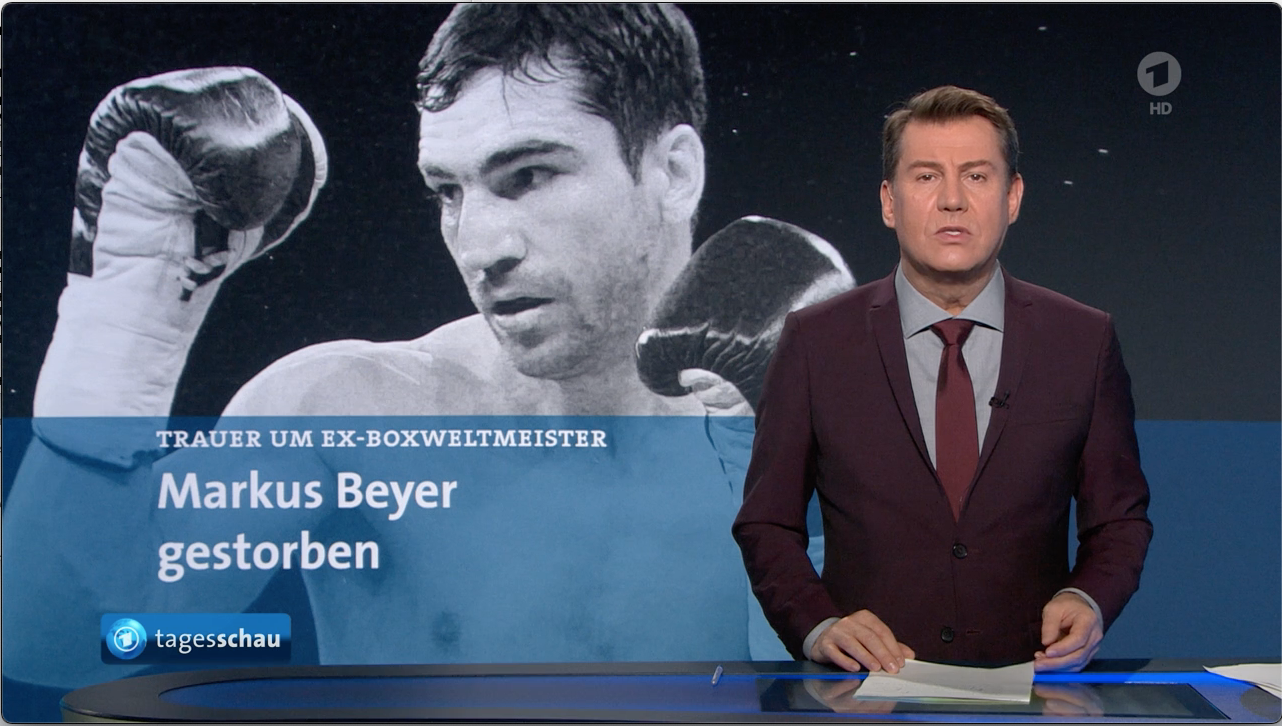
\includegraphics[width=.7\textwidth]{Figures/Bildschirmfoto-Markus-Beyer.png}}}

\vfill
%\movie[options]{placeholder box}{movie filename}

%\movie{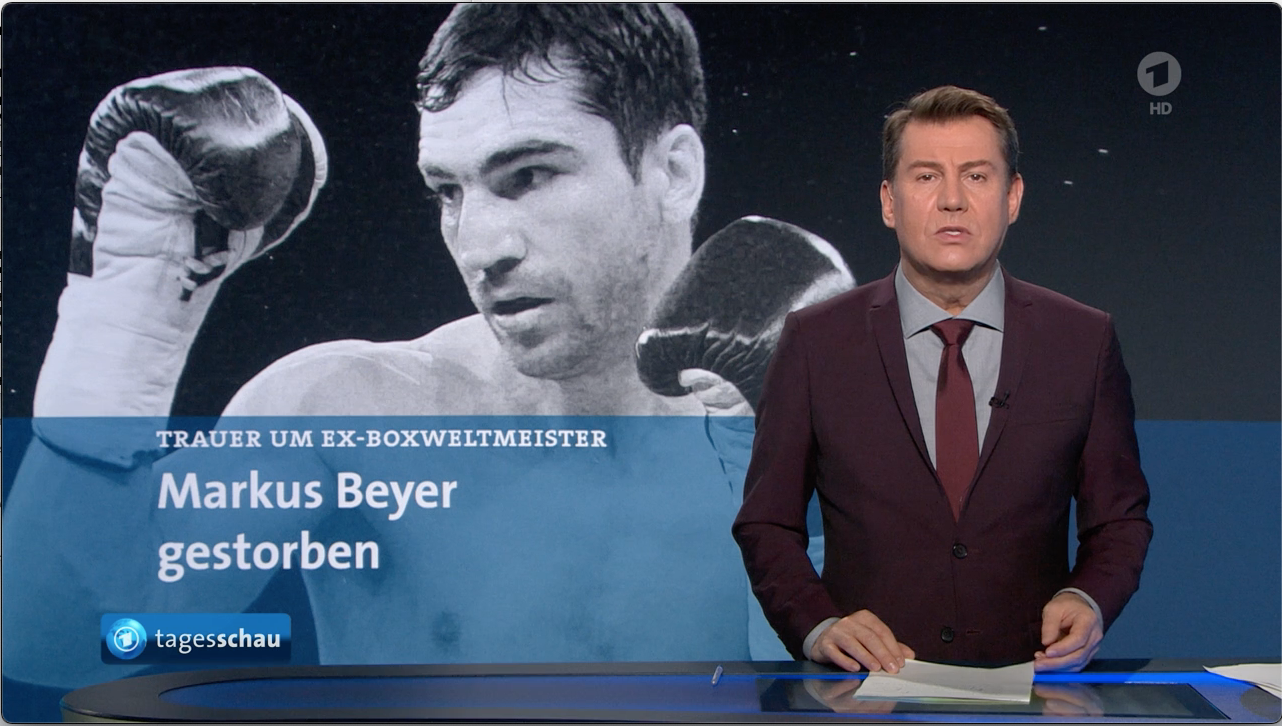
\includegraphics[width=.7\textwidth]{Figures/Bildschirmfoto-Markus-Beyer.png}}{Mehrfach-VF-zum-ersten-Mal-Weltmeister-TV-20181204-2015-4401-webxl-h264.mp4}

\pause
\ea
Zum ersten Mal Weltmeister wurde er vor 19 Jahren.\footnote{
  tagesschau, 04.12.2018, 20:00.
}
\z

\vfill

}

% \frame{
% \frametitle{And now for something completely different}

% \vfill

% %\centerline{\href{run:./Mehrfach-VF-zum-ersten-Mal-Weltmeister-TV-20181204-2015-4401-webxl-h264.mp4}{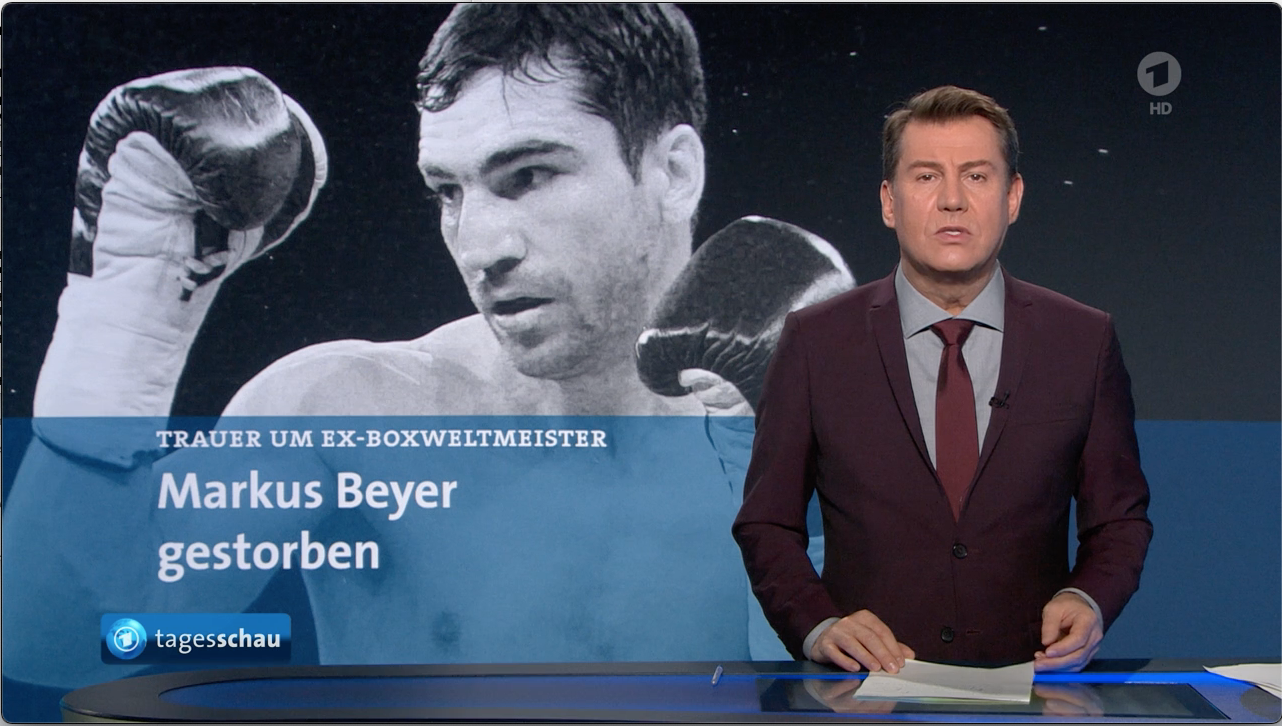
\includegraphics[width=.7\textwidth]{Figures/Bildschirmfoto-Markus-Beyer.png}}}

% % \includemovie{.85\textheight}{.85\textheight}{Mehrfach-VF-zum-ersten-Mal-Weltmeister-TV-20181204-2015-4401-webxl-h264.mp4}%

% \vfill
% %\movie[options]{placeholder box}{movie filename}

% %\movie{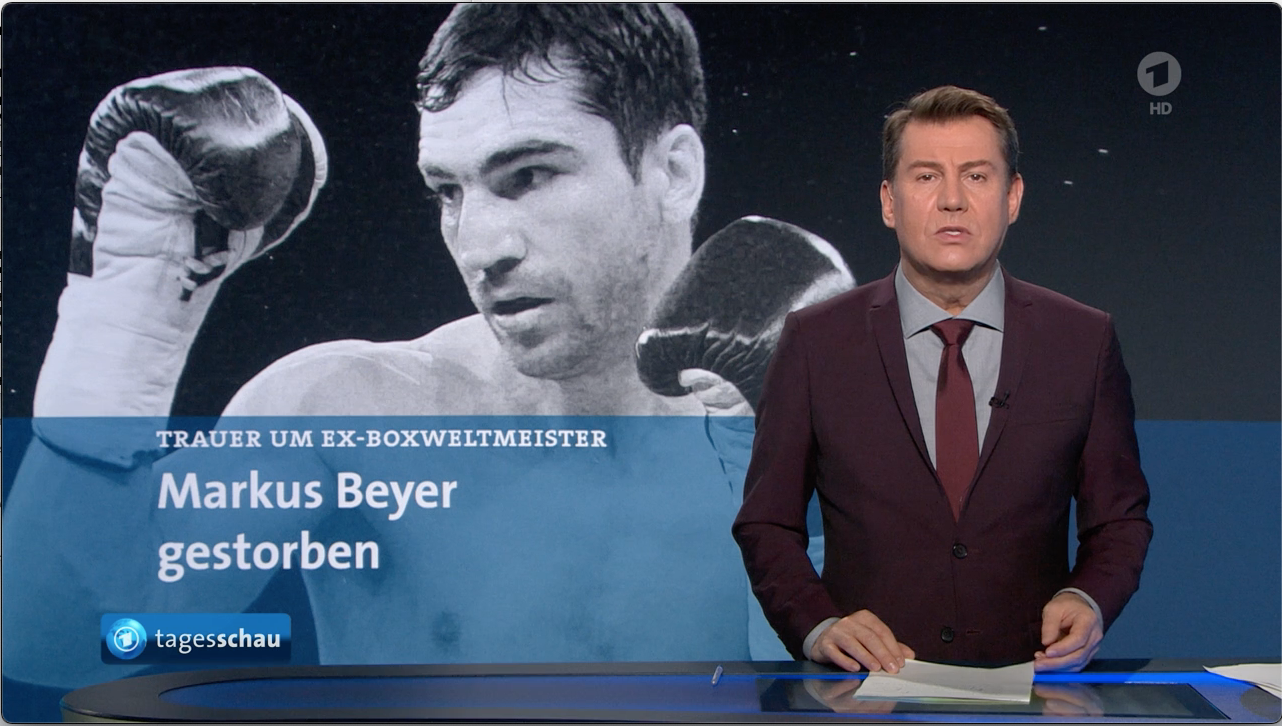
\includegraphics[width=.7\textwidth]{Figures/Bildschirmfoto-Markus-Beyer.png}}{Mehrfach-VF-zum-ersten-Mal-Weltmeister-TV-20181204-2015-4401-webxl-h264.mp4}

% \pause
% \ea
% Zum ersten Mal Weltmeister wurde er vor 19 Jahren.\footnote{
%   tagesschau, 04.12.2018, 20:00.
% }
% \z

% \vfill

% }



\frame{
\frametitle{Probleme mit flachen Strukturen: Mehrfache VF-Besetzung}
\savespace

\begin{itemize}
\item Sätze wie (\mex{1}) können mit leerem Kopf gut erklärt werden:
\eal
%% \ex Fachleute erkennen Salzschäden an Bäumen relativ gut. [\ldots] Es kann also einige
%%     Winterperioden dauern, bis man den Effekt beobachten kann. [\ldots] [Exakt] [auf das Salz]
%%     kann man es tatsächlich erst zurückführen, wenn es für den Baum zu spät ist.\footnote{
%%         taz berlin, 22.12.2003, S.\,22
%%     }
\ex {}[Dauerhaft] [mehr Arbeitsplätze] gebe es erst, wenn sich eine Wachstumsrate von
      mindestens 2,5 Prozent über einen Zeitraum von drei oder vier Jahren halten lasse.\footnote{
        taz, 19.04.2000, S.\,5 %taz Nr. 6123 vom 19.4.2000 Seite 5
      }
\ex Unverhohlen verärgert auf Kronewetters Vorwurf reagierte Silke Fischer.\footnote{
    taz berlin, 23.04.2004, S.\,21
}
\ex {}[Hart] [ins Gericht] ging Klug mit dem Studienkontenmodell der Landesregierung.\footnote{
  taz nord, 19.02.2004, S.\,24
  }
\zl
\pause
\item weitere Daten in \citew{Mueller2003b,Bildhauer2011a,MuellerGS}

\pause
\item Ohne leeren Kopf nicht erklärbar oder nur mit Stipulationen.
\end{itemize}
}

\subsubsection{Binär verzweigende Strukturen und Linearisierungsdomänen}


\frame{

\footnotesize
\frametitlefit{Linearisierungsdomänen und diskontinuierliche Konstituenten}

\medskip


\centerline{%
\alt<handout>{%
\begin{forest}
sm edges
[{V[\subcat \sliste{} ]}
  [\blau{\ibox{1} NP[\type{nom}]},ellipse,draw
    [Aicke]]
  [{V[\subcat \sliste{ \ibox{1} }]}
    [\blau{\ibox{2} NP[\type{acc}]},ellipse,draw 
      [Futter, roof]]
    [{V[\subcat \sliste{ \ibox{1}, \ibox{2} }]}
      [\blau{\ibox{3} NP[\type{dat}]},ellipse,draw
        [dem Affen,roof]]
      [\blau{V[\subcat \sliste{ \ibox{1}, \ibox{2}, \ibox{3} }]},ellipse,draw
        [gibt]]]]]
\end{forest}}{
\begin{forest}
sm edges
[{V[\subcat \sliste{} ]}
  [\blau{\ibox{1} NP[\type{nom}]}
    [Aicke]]
  [{V[\subcat \sliste{ \ibox{1} }]}
    [\blau{\ibox{2} NP[\type{acc}]}
      [Futter, roof]]
    [{V[\subcat \sliste{ \ibox{1}, \ibox{2} }]}
      [\blau{\ibox{3} NP[\type{dat}]}
        [dem Affen,roof]]
      [\blau{V[\subcat \sliste{ \ibox{1}, \ibox{2}, \ibox{3} }]}
        [gibt]]]]]
\end{forest}}
}


\begin{itemize}[<+->]
\item \alt<handout>{eingekreiste}{blaue} Knoten werden in eine Liste eingefügt: die Linearisierungsdomäne
\item die Permutation von Elementen in solchen Domänen ist nur durch Linearisierungsregeln beschränkt
\item Linearisierungsdomänen sind Kopfdomänen $\leftrightarrow$ {\it Scrambling\/} ist lokal
\end{itemize}

}

\frame{


\frametitle{Repräsentation lexikalischer Köpfe}


\hspace{4mm}
\ms[word]{
phon & \ibox{1} \\
synsem & \ibox{2} \\
dom & \liste{ \ms[word]{ phon & \ibox{1} \\
                                 synsem & \ibox{2} \\
                                 dom    & \liste{}\\
                               }
            } \\
}
\begin{itemize}[<+->]
\item Jeder Kopf enthält in seiner Konstituentenstellungsdomäne eine Beschreibung von sich selbst.
\item Adjunkt- und Komplementtöchter werden in diese Liste eingesetzt und relativ zu ihm angeordnet.
\end{itemize}

}

\pdfbookmark[5]{Domänenbildung}{domain-formation}
\frame[shrink]{

\smallframe\parskip0pt\itemsep0pt
\frametitle{Domänenbildung}
\begin{itemize}
\item alle Nicht"=Kopftöchter werden in die Domäne des Kopfes eingesetzt

\type{head-non-cluster-phrase} \impl

\ms{
  head-dtr$|$dom  & \ibox{1} \\
  non-head-dtrs   & \ibox{2} \\
  dom  & \ibox{1} $\bigcirc$ \ibox{2} \\
}
\item Dort können sie frei angeordnet werden, solange LP"=Regeln nicht verletzt sind.

\item Die {\it shuffle\/}"=Relation besteht zwischen drei Listen
A, B und C, gdw.\ C alle Elemente von A und B enthält und die Reihenfolge
der Elemente von A und die Reihenfolge der Elemente in B in C erhalten ist.

$\phonliste{ a, b } \bigcirc \phonliste{ c, d } =
\begin{tabular}[t]{@{}l}
\phonliste{ a, b, c, d } $\vee$\\*
\phonliste{ a, c, b, d } $\vee$\\*
\phonliste{ a, c, d, b } $\vee$\\*
\phonliste{ c, a, b, d } $\vee$\\*
\phonliste{ c, a, d, b } $\vee$\\*
\phonliste{ c, d, a, b }
\end{tabular}$
\end{itemize}

}

\frame{
\pdfbookmark[5]{PHON-Berechnung}{phon-computation}
\frametitle{{\sc phon}-Berechnung}
\begin{itemize}
\item in Domäne entsprechend der Oberflächenreihenfolge angeordnet
\item $\to$ Berechnung des {\sc phon}"=Wertes ist einfache Konkatenation

\medskip
\ms[phrase]{
 phon & \ibox{1} $\oplus$ \ldots $\oplus$ \ibox{n} \\ \\
     dom  & \liste{ \ms[sign]{ phon & \ibox{1} \\ }, \ldots, \ms[sign]{ phon & \ibox{n} \\ }
                  } \\
   }
\end{itemize}

}

\subsubsection{Beispiele}

\frame{

\frametitle{Beispiel: Kontinuierliche Konstituenten}

\begin{forest}
sm edges
[V\feattab{\subcat \sliste{},\\
           \textsc{dom} \phonliste{ Aicke, dem Affen, den Stock, gibt }}
  [{\ibox{1} NP[\type{nom}]}
    [Aicke,roof]]
  [V\feattab{\subcat \sliste{ \ibox{1} },\\
             \textsc{dom} \phonliste{ dem Affen, den Stock, gibt }}
    [{\ibox{2} NP[\type{dat}]} 
      [dem Affen, roof]]
    [V\feattab{\subcat \sliste{ \ibox{1}, \ibox{2} },\\
               \textsc{dom} \phonliste{ den Stock, gibt }}
      [{\ibox{3} NP[\type{acc}]}
        [den Stock,roof]]
      [V\feattab{\subcat \sliste{ \ibox{1}, \ibox{2}, \ibox{3} },\\
        \textsc{dom} \phonliste{ gibt }}
        [gibt]]]]]
\end{forest}

}

\frame{

\frametitlefit{Beispiel: Diskontinuierliche Konstituenten / Anordnung im \mf}

\begin{forest}
sm edges
[V\feattab{\subcat \sliste{},\\
           \textsc{dom} \phonliste{ Aicke, \blau{den Stock}, dem Affen, \blau{gibt} }}
  [{\ibox{1} NP[\type{nom}]}
    [Aicke,roof]]
  [V\feattab{\subcat \sliste{ \ibox{1} },\\
             \textsc{dom} \phonliste{ \blau{den Stock}, dem Affen, \blau{gibt} }}
    [{\ibox{2} NP[\type{dat}]} 
      [dem Affen, roof]]
    [V\feattab{\subcat \sliste{ \ibox{1}, \ibox{2} },\\
               \textsc{dom} \phonliste{ \blau{den Stock, gibt} }}
      [{\ibox{3} NP[\type{acc}]}
        [den Stock,roof]]
      [V\feattab{\subcat \sliste{ \ibox{1}, \ibox{2}, \ibox{3} },\\
        \textsc{dom} \phonliste{ gibt }}
        [gibt]]]]]
\end{forest}
}

\frame{

\frametitlefit{Beispiel: Diskontinuierliche Konstituenten / Verberststellung}


\begin{forest}
sm edges
[V\feattab{\subcat \sliste{},\\
           \textsc{dom} \phonliste{ \blau{gibt}, Aicke, dem Affen, \blau{den Stock} }}
  [{\ibox{1} NP[\type{nom}]}
    [Aicke,roof]]
  [V\feattab{\subcat \sliste{ \ibox{1} },\\
             \textsc{dom} \phonliste{ \blau{gibt}, dem Affen, \blau{den Stock} }}
    [{\ibox{2} NP[\type{dat}]} 
      [dem Affen, roof]]
    [V\feattab{\subcat \sliste{ \ibox{1}, \ibox{2} },\\
               \textsc{dom} \phonliste{ \blau{gibt, den Stock} }}
      [{\ibox{3} NP[\type{acc}]}
        [den Stock,roof]]
      [V\feattab{\subcat \sliste{ \ibox{1}, \ibox{2}, \ibox{3} },\\
        \textsc{dom} \phonliste{ gibt }}
        [gibt]]]]]
\end{forest}

}

%\fi
\frame{
\frametitlefit{Verbstellung mit den Konstituenten in Oberflächenreihenfolge}


% \forestset{
%   default preamble'={}, % The default preamble makes a mess in this situation.
%   % 
%   % This style visually relates a complement to some subcat node. The argument
%   % should be the intended SISTER.
%   funky complement/.style={
%     %tier=NP, % Horizontally align NPs ... not needed because they are all of the same height.
%     for children={tier=word}, % Align the NP content with "gibt".
%     for nodewalk/.process=Ow{#1.id}{id=##1}{% This monstrosity converts a relative node name (e.g. "!r1") to the id of that node.
%       edge label={node[pos=0.5,left]{H}}, % Put "H" on the edge from the sister subcat.
%     },
%     % Draw the funky edge from a complement to its visual parent. The line is
%     % broken at the north of the sister subcat, and also marked with "C" there.
%     edge path'={(#1u.south) -- (.north |- {#1.north}) node[above]{C} -- (.north)},
%   },
% }
% \begin{forest}
%   % sn edges,   % note the s*n*, not s*m* // Can live without, as we draw the funky edges manually.
%   for tree={l sep*=2}, % Let this tree be taller.
%   [V\feattab{\subcat \sliste{},\\
%       \textsc{dom} \phonliste{ gibt, der Mann, das Buch, der Frau }}
%     [V\feattab{\subcat \sliste{ \ibox{1} },\\
%         \textsc{dom} \phonliste{ gibt, bas Buch, der Frau }},
%       [V\feattab{\subcat \sliste{ \ibox{1}, \ibox{2} },\\
%           \textsc{dom} \phonliste{ gibt, der Frau }}
%         [V\feattab{\subcat \sliste{ \ibox{1}, \ibox{2}, \ibox{3} },\\
%             \textsc{dom} \phonliste{ gibt }},
%           [gibt]]]]
%     [,% This empty node holds all the complements. The idea is to put it next
%       % to the subcat node that should determine the x (s) position of the
%       % complements (so I put it next to the second subcat node). How does this
%       % work? On its own, Forest squashes the complements close to "gibt", but
%       % then the funky edge from NP [1] overlaps the second subcat node. But
%       % then we adjust the "s" of this empty complement holder (in "before
%       %   computing xy") to avoid that.
%       no edge, % Phantom does not work here, because we need the empty
%                % complement holder to be physically present.
%       calign=first, % Put this empty node directly above the leftmost NP ...
%       before computing xy={% ... and set its position manually:
%         %s/.option={!s.max x}, % to the (right) width of its sibling (the second subcat)
%         %s+/.option=!u.s sep,  % plus a bit more
%       },
%       tier=lowest subcat, % Vertically align it to the lowest subcat node (gibt).
%       for parent={calign=first}, % The sister subcat (Buch, Frau) should be
%                                  % directly below its parent.
%       for sibling={where n children=0{% This finds "gibt".
%           for parent={tier=lowest subcat}, % Mark the lowest subcat for alignment with the empty complement holder.
%           tier=word, % Align "gibt" with the content of NPs.
%         }{}},
%       [{\ibox{1} NP[\type{nom}]}, funky complement=!r1 % the first child of the root
%         [der Mann,roof]]
%       [{\ibox{1} NP[\type{acc}]}, funky complement=!r11  % the first child of the first child of the root
%         [das Buch,roof]]
%       [{\ibox{1} NP[\type{dat}]}, funky complement=!r111
%         [der Frau,roof]]]
%   ]
% \end{forest}

\vfill
\centerline{\includegraphics[scale=.7]{Figures/fig-domains-discont}}
\vfill

% \forestset{
% %  default preamble'={}, % The default preamble makes a mess in this situation.
%   % 
%   % This style visually relates a complement to some subcat node. The argument
%   % should be the intended SISTER.
%   funky complement/.style={
%     %tier=NP, % Horizontally align NPs ... not needed because they are all of the same height.
%     for children={tier=word}, % Align the NP content with "gibt".
%     for nodewalk/.process=Ow{#1.id}{id=##1}{% This monstrosity converts a relative node name (e.g. "!r1") to the id of that node.
%       edge label={node[pos=0.5,left]{H}}, % Put "H" on the edge from the sister subcat.
%     },
%     % Draw the funky edge from a complement to its visual parent. The line is
%     % broken at the north of the sister subcat, and also marked with "C" there.
%     edge path'={(#1u.south) -- (.north |- {#1.north}) node[above]{C} -- (.north)},
%   },
% }
% \begin{forest}
%   % sn edges,   % note the s*n*, not s*m* // Can live without, as we draw the funky edges manually.
%   for tree={l sep*=2}, % Let this tree be taller.
% delay={where tier={word}{inner xsep=0}{}}, % unclear why it has to happen here with delay.
%   [V\feattab{\subcat \sliste{},\\
%       \textsc{dom} \phonliste{ gibt, Aicke, dem Affen, den Stock }}, s sep+=7ex
%     [V\feattab{\subcat \sliste{ \ibox{1} },\\
%         \textsc{dom} \phonliste{ gibt, dem Affen, den Stock }},
%       [V\feattab{\subcat \sliste{ \ibox{1}, \ibox{2} },\\
%           \textsc{dom} \phonliste{ gibt, den Stock }}
%         [V\feattab{\subcat \sliste{ \ibox{1}, \ibox{2}, \ibox{3} },\\
%             \textsc{dom} \phonliste{ gibt }},
%           [gibt]]]]
%     [,% This empty node holds all the complements. The idea is to put it next
%       % to the subcat node that should determine the x (s) position of the
%       % complements (so I put it next to the second subcat node). How does this
%       % work? On its own, Forest squashes the complements close to "gibt", but
%       % then the funky edge from NP [1] overlaps the second subcat node. But
%       % then we adjust the "s" of this empty complement holder (in "before
%       %   computing xy") to avoid that.
%       no edge, % Phantom does not work here, because we need the empty
%                % complement holder to be physically present.
%       calign=first, % Put this empty node directly above the leftmost NP ...
%       before computing xy={% ... and set its position manually:
%         %s/.option={!s.max x}, % to the (right) width of its sibling (the second subcat)
%         %s+/.option=!u.s sep,  % plus a bit more
%       },
%       tier=lowest subcat, % Vertically align it to the lowest subcat node (gibt).
%       for parent={calign=first}, % The sister subcat (Buch, Frau) should be
%                                  % directly below its parent.
%       for sibling={where n children=0{% This finds "gibt".
%           for parent={tier=lowest subcat}, % Mark the lowest subcat for alignment with the empty complement holder.
%           tier=word, % Align "gibt" with the content of NPs.
%           %inner xsep=0, % Remove space otherwise the triangles get too big.
%           % Does not work here, has to be done with delay at the top. St. Mü. 21.06.2024
%         }{}},
%       [{\ibox{1} NP[\type{nom}]}, funky complement=!r1 % the first child of the root
%         [Aicke,roof]]
%       [{\ibox{2} NP[\type{dat}]}, funky complement=!r11  % the first child of the first child of the root
%         [dem Affen,roof]]
%       [{\ibox{3} NP[\type{acc}]}, funky complement=!r111
%         [den Stock,roof]]]
%   ]
% \end{forest}

}

%\if0
\frame{
\frametitle{Eine Anmerkung}



\begin{itemize}
\item die Dominanzstrukturen für die Folgen in (\mex{1}) sind identisch:
      \eal
      \ex der Delphin dem Kind den Ball gibt
      \ex der Delphin den Ball dem Kind gibt
      \ex Gibt der Delphin den Ball dem Kind?
      \zl
\item Nur die Anordnung der Elemente in den Stellungsdomänen ist anders.
\end{itemize}




}


\subsubsection{Probleme der Linearisierungsansätze}
\frame{
\frametitle{Probleme der Linearisierungsansätze}

\begin{itemize}
\item Diese Ansätze haben denselben Nachteil, wie die Ansätze,\\
      die von flachen Strukturen ausgehen:
Man kann nicht motivieren,\\
dass mehrere Konstituenten im Vorfeld eine gemeinsame Konstituente bilden.
\end{itemize}
}

\frame{
\frametitlefit{Probleme der Linearisierungsansätze: Teilprojektionen im VF}

\savespace
\begin{itemize}
\item Man kann nicht ohne weiteres erklären,
wieso sowohl Dativobjekte als auch Akkusativobjekte mit dem Verb im Vorfeld stehen können.
\eal
\ex Den Wählern erzählen sollte man diese Geschichte nicht.
\ex Märchen erzählen sollte man den Wählern nicht.
\zl
\pause
\item In Linearisierungsgrammatiken muss man die Argumente eines Kopfes
in einer festen Reihenfolge sättigen, da die Sättigungsreihenfolge von der Oberflächenreihenfolge unabhängig ist.
\pause
\item mit \subcatl $\langle$ NP[{\it nom}], NP[{\it acc}], NP[{\it dat}] $\rangle$ nur (\mex{0}a) analysierbar\\
(\mex{0}b) bleibt unanalysierbar, da \emph{Märchen} erst mit \emph{erzählen} kombiniert werden kann, wenn die Kombination
mit dem Dativobjekt erfolgt ist.

\pause
\item \citet{Kathol2000a}: keine Reihenfolge für Objekte in der \subcatl\\
Damit sind Sätze in (\mex{0}) analysierbar, aber (\mex{1}) hätte zwei Analysen:
\ea
dass er den Wählern Märchen erzählt
\z
\end{itemize}
}

\frame{
\frametitle{Teilprojektionen im VF}

\begin{itemize}
\item Für den hier vorgestellten Ansatz sind  Sätze in (\mex{1}) unproblematisch:
\eal
\ex Den Wählern erzählen sollte man diese Geschichte nicht.
\ex Märchen erzählen sollte man den Wählern nicht.
\zl
Das Kopf"=Argument"=Schema läßt Kombination von Argumenten mit ihrem Kopf in beliebiger Reihenfolge zu. \compare{pvp}{Voranstellung von Phrasenteilen}
\end{itemize}
}


\subsubsection{Variable Verzweigung}

\frame{
\frametitle{Variable Verzweigung}

\begin{itemize}
\item \citet{Crysmann2003b}, \citet{KW91a} und \citet{SRTD96a}

unterschiedliche Verzweigungen:
\eal
\ex {}[[[Gibt er] dem Mann] den Ball]?
\ex {}[Hat [er [dem Mann [den Ball gegeben]]]]?
\zl
\pause
\item keinen leeren verbalen Kopf 
\pause
\item keine Möglichkeit, die scheinbar mehrfache
Vorfeldbesetzung mit Hilfe eines leeren verbalen Kopfes zu erklären
\end{itemize}

}

\subsubsection{Zusammenfassung}

\frame{
\frametitle{Zusammenfassung}

\begin{itemize}[<+->]
\item Es sieht so aus, als würde man wirklich eine GB-artige Analyse der deutschen Satzstellung
  brauchen.
\item Verbspur am Ende des Satzes.\\
      Finites Verb analog zum Komplementierer in Erststellung.

\end{itemize}

\pause\pause\pause

}


} % \end{teil1}

%\fi

